\documentclass[11pt,a4paper]{article}
\usepackage[margin=0.86in,headheight=14pt]{geometry}
\usepackage[T1]{fontenc}
\usepackage[utf8]{inputenc}
\usepackage{lmodern}
\usepackage{microtype}
\usepackage{graphicx}
\usepackage{booktabs,tabularx,longtable,array}
\usepackage{enumitem}
\usepackage{xcolor}
\usepackage{hyperref}
\usepackage{fancyhdr}
\usepackage[most]{tcolorbox}
\usepackage{titlesec}
\usepackage{listings}
\usepackage{amsmath,amssymb}
\usepackage{tikz}
\usetikzlibrary{arrows.meta,positioning,shapes.geometric}
\definecolor{ink}{HTML}{14253B}
\definecolor{navy}{HTML}{183858}
\definecolor{teal}{HTML}{007E83}
\definecolor{pale}{HTML}{F0F5F7}
\definecolor{muted}{HTML}{506276}
\definecolor{gold}{HTML}{DAA650}
\hypersetup{colorlinks=true,urlcolor=teal,linkcolor=navy,citecolor=teal,pdftitle={Memorize, Retrieve, or Query? Course Research Roadmap},pdfauthor={Research Project Planning Document}}
\pagestyle{fancy}\fancyhf{}\lhead{\small\color{muted}Memorize, Retrieve, or Query?}\rhead{\small\color{muted}Course research roadmap}\cfoot{\small\thepage}
\titleformat{\section}{\Large\bfseries\color{navy}}{\thesection}{0.7em}{}
\titleformat{\subsection}{\large\bfseries\color{navy}}{\thesubsection}{0.7em}{}
\titleformat{\subsubsection}{\normalsize\bfseries\color{teal}}{\thesubsubsection}{0.6em}{}
\setlist[itemize]{leftmargin=1.5em,topsep=2pt,itemsep=2pt}
\setlist[enumerate]{leftmargin=1.7em,topsep=2pt,itemsep=3pt}
\setlength{\parskip}{5pt}\setlength{\parindent}{0pt}
\newtcolorbox{keybox}[1][]{colback=pale,colframe=teal!65!black,boxrule=0.5pt,arc=2mm,left=9pt,right=9pt,top=7pt,bottom=7pt,#1}
\newtcolorbox{warnbox}[1][]{colback=gold!8,colframe=gold!75!black,boxrule=0.5pt,arc=2mm,left=9pt,right=9pt,top=7pt,bottom=7pt,#1}
\lstdefinestyle{compact}{basicstyle=\ttfamily\scriptsize,breaklines=true,columns=fullflexible,showstringspaces=false,frame=single,rulecolor=\color{muted!30},backgroundcolor=\color{pale},numbers=none,aboveskip=5pt,belowskip=5pt}
\lstset{style=compact}
\newcommand{\deliver}[1]{\textbf{Output:} #1}
\newcommand{\gate}[1]{\textbf{Acceptance gate:} #1}
\begin{document}
\begin{titlepage}
\vspace*{1.1cm}
{\color{teal}\rule{\linewidth}{2.5pt}}\\[0.65cm]
{\Huge\bfseries\color{navy}Memorize, Retrieve,\\[0.12cm]or Query?}\\[0.36cm]
{\LARGE\color{muted}LLMs answering questions about\\a software project's history}\\[0.8cm]
{\Large\bfseries A practical, reproducible course research roadmap}\\[0.25cm]
{\normalsize Problem definition \textbullet\ Literature \textbullet\ Data \textbullet\ Systems \textbullet\ Evaluation \textbullet\ Timeline}
\vfill
\begin{keybox}
\textbf{Recommended minimum viable study:} One Mozilla Bugzilla project scope; a curated, frozen historical bug corpus; six question families; four primary approaches plus an optional router; one common freely accessible language model; and a \emph{time-controlled} update experiment. Build the benchmark and deterministic ground truth before building a polished chatbot.
\end{keybox}
\vspace{0.5cm}
\begin{tabularx}{\linewidth}{@{}lX@{}}
\textbf{Audience} & Course project team and instructor \\
\textbf{Planning horizon} & Eight weeks (compressible to six) \\
\textbf{Budget target} & \$0 in API charges and software licenses (local hardware/internet excluded) \\
\textbf{Research snapshot} & 21 October 2026; verify free-model eligibility and data endpoints at execution time \\
\textbf{Document type} & Research/implementation plan, not evidence of completed experiments \\
\end{tabularx}
\vspace{0.5cm}
{\color{teal}\rule{\linewidth}{1pt}}
\end{titlepage}
\setcounter{tocdepth}{1}\tableofcontents\clearpage

\section{The problem in simple terms}
Imagine joining the Firefox team and asking: \emph{``How long did bug 12345 take to get fixed, which component owned it, and why did it take so long?''} The answer may be distributed across a bug's creation date, status transitions, comments, and possibly a linked source-code change. A general chatbot may guess; ordinary search may find the right bug but miss the exact resolution event; a database can calculate the duration precisely but cannot always summarize discussions.

We will create a \emph{research prototype} that accepts natural-language questions about Mozilla bug history, retrieves or computes evidence, returns a concise answer, and shows its sources. Its purpose is \textbf{not} to become a production Firefox support product. Its purpose is to learn which method works best for which kinds of questions, when it invents unsupported facts, and how it behaves when new records arrive.

\begin{keybox}
\textbf{The crucial distinction:} ``Time to resolve'' is the elapsed calendar interval from filing to a defined status/resolution event. It is \emph{not} engineering effort, active developer hours, or necessarily the date a patch was merged. A bug may be reopened, duplicate-closed, or never fixed. Definitions must be explicit before testing.
\end{keybox}

\subsection{A complete example}
Suppose a \emph{fictional} bug was opened on 1 March at 09:00 UTC and first changed to RESOLVED/FIXED on 5 March at 15:00 UTC. The mathematically supported answer is \textbf{4 days and 6 hours to first FIXED}. An LLM that outputs ``4 days'' loses precision; an LLM that claims ``the developer spent 4 days fixing it'' confuses elapsed time with labor. A fully cited system would show the bug ID and the two recorded events. If a user asks \emph{why}, the system needs corroborating comments and should not infer causal reasons without them.

\subsection{Research objective and non-goals}
\textbf{Objective:} Empirically compare parametric answering, document retrieval, hybrid retrieval, deterministic structured querying, and a lightweight relationship-aware approach on verifiable Mozilla issue-history questions under static and updated data snapshots.

\textbf{Non-goals:} Train an LLM from scratch, guarantee the cause of a bug, estimate actual person-hours without timesheets, model all Firefox source code, run a production cluster, or recreate Microsoft's complete LLM-extracted GraphRAG pipeline. Linked commits are \emph{optional} enrichment, not a guaranteed field from Bugzilla REST.

\section{Exactly what the team should deliver}
\begin{longtable}{@{}p{0.05\linewidth}p{0.30\linewidth}p{0.56\linewidth}@{}}
\toprule
\textbf{ID}&\textbf{Artifact}&\textbf{Minimum evidence it must contain}\\ \midrule\endhead
D1&Written proposal and RQs&Problem, novelty boundary, formal terms, hypotheses, project scope.\\
D2&Data pipeline and manifest&Reproducible extraction/import; Bugzilla schema; source URLs; timestamps; counts; deduplication and quality report.\\
D3&Versioned benchmark&180 proposed QA items; 36 development and 144 locked test; gold answers, evidence, temporal cutoff, question type and rubric.\\
D4&Four implemented comparators&Closed-book LLM; BM25-RAG; hybrid RAG; read-only structured-query/SQL approach. One extra lightweight KG traversal variant if time allows.\\
D5&Unified question answering UI&Local Streamlit chat, selectable method, text response, bug IDs/links, timestamp of corpus snapshot, expandable evidence and latency.\\
D6&Experiment records&Frozen model/config; JSONL predictions; retrieved evidence, structured-query trace, abstentions, timings and token/request usage.\\
D7&Evaluation tables and plots&Per-family correctness, hallucination, evidence support, answerability, latency; temporal degradation and update recovery, confidence intervals.\\
D8&Report and presentation&Related work and limitation statement; method diagram; results; failure cases; replication instructions; demo script.\\ \bottomrule
\end{longtable}
\begin{warnbox}
\textbf{Priority order:} D2 $\rightarrow$ D3 $\rightarrow$ D4 $\rightarrow$ D6--D7 $\rightarrow$ D5. A convincing benchmark with honest results is more important than a beautiful interface without a valid test set.
\end{warnbox}

\section{What is already known? Literature and novelty check}
This topic is \textbf{not new as a generic ``ask a software repository'' chatbot}. The closest works below should be discussed early in the proposal instead of claiming first-ever repository Q\&A.

\begin{longtable}{@{}p{0.28\linewidth}p{0.34\linewidth}p{0.29\linewidth}@{}}
\toprule \textbf{Work}&\textbf{What it established}&\textbf{How our course study differs}\\\midrule\endhead
\textbf{RepoChat} (Abedu et al., MSR 2025)\cite{repochat}&LLM translates repository questions to knowledge-graph queries and produces answers; evaluated through a user study.&Compare \emph{multiple} architectures on Bugzilla \emph{history} questions, with specific drift and evidence checks.\\
\textbf{Synergizing LLMs and KGs} (Abedu et al., ACM TOSEM 2026)\cite{abedu}&In-depth repository Q\&A with graph + LLM and varied question complexity.&Avoid presenting KG--LLM Q\&A as novel; assess historical snapshots, quantitative dates, unsupported answers and incremental updates.\\
\textbf{KG+RAG for past service tickets} (Xu et al., 2024)\cite{xukgrag}&Uses relationships within and between historical tickets for technical support Q\&A.&Shows ticket-oriented KG+RAG is already explored; motivate a domain-specific comparative benchmark.\\
\textbf{GraphRAG} (Edge et al., 2024)\cite{edgerag}&Graph-structured indexing for global, corpus-wide summaries.&A full generative graph construction is expensive and not essential for precise lifecycle questions.\\
\textbf{Temporal KG QA survey} (Su et al., 2024)\cite{temporalkg}&Describes temporal questions and reasoning over evolving structured knowledge.&Justifies explicit ``as-of'' constraints, event sequences and timestamp-aware evaluation.\\
\textbf{BugsRepo} (Acharya and Ginde, 2025)\cite{bugsrepo}&Curated Mozilla Bugzilla metadata and comments, useful as input data.&Dataset is a \emph{source}, not our answer benchmark; gold answers and time-controlled tests must be constructed.\\
\textbf{RAGAS} (Es et al., 2023)\cite{ragas}&Evaluation decomposes retrieval quality, faithfulness and answer relevance.&Use as inspiration, not the sole judge; verified timestamps and claims take precedence.\\
\bottomrule
\end{longtable}

\textbf{Defensible contribution:} ``A controlled benchmark and failure analysis of closed-book, retrieval-based, relationship-aware and executable-query methods on Mozilla Bugzilla history, including temporal knowledge updates.'' Novelty is in the \emph{question taxonomy, temporal protocol, answerability/grounding rubric and paired comparisons}, not in inventing RAG or KGs.

\textbf{Literature task (week 1):} Read the abstracts, methods, datasets and evaluation sections of the first three papers closely. Make a one-page matrix showing: data sources, question categories, models, gold-answer mechanism, temporal treatment and hallucination metrics. Search once more immediately before final submission for a closer study; do not make absolute novelty claims.

\section{Research questions, hypotheses and boundaries}
\textbf{RQ1---Method by question type.} How do closed-book LLM, BM25-RAG, hybrid RAG and structured-query approaches differ in answer correctness across bug lookup, lifecycle timing, corpus aggregation, cross-record linking, explanation and unanswerable questions?

\textbf{RQ2---Grounding and hallucination.} Which approaches produce the highest proportion of supported factual claims, verifiable citations, and correct abstentions when records are missing or ambiguous?

\textbf{RQ3---Temporal robustness.} How much performance is lost when systems remain frozen after a controlled data cutoff, and how much is recovered when their indexes or structured stores are refreshed with the same new bug events?

\textbf{Optional RQ4---Routing.} Does choosing a deterministic query for numeric/temporal questions and retrieval for explanatory questions improve accuracy--latency trade-offs over one uniform approach?

\begin{tabularx}{\linewidth}{@{}p{0.13\linewidth}X@{}}
\toprule H1 & Structured queries outperform retrieval-only approaches on exact durations, counts and status-history comparisons when records are complete.\\
H2 & Retrieval-grounded approaches outperform closed-book answering on evidence-driven explanations, but can still hallucinate if retrieval misses necessary events.\\
H3 & Frozen external knowledge causes poorer results on post-cutoff questions; refreshing indexes/stores helps, though the size of improvement depends on question type.\\
H4 (optional)& A simple query router achieves higher factual correctness without needing a fully agentic system.\\\bottomrule
\end{tabularx}

\textbf{Pre-register:} primary endpoint = question-level exact/semantic correctness (as defined per family); secondary = unsupported-claim rate, correctly supported answer rate, citation precision, correct abstention, retrieval Recall@k, p50/p95 latency and update benefit. Results should include negative findings.

\section{Choosing the data: Mozilla, BugsRepo and the REST API}
\subsection{Recommended two-source strategy}
\textbf{Source A---BugsRepo,} as a reusable historical seed: the authors report 119,585 resolved/fixed-or-closed bug records and comments across more than 50 Mozilla projects, snapshot circa October 2024, plus contributor data (19,351 members) and a structured subset (10,351 bugs)\cite{bugsrepo}. Zenodo record \url{https://zenodo.org/records/15004067} contains a roughly 4.3-GB publication bundle. Start with the smaller metadata/structured CSVs or sample, not the entire multi-GB corpus.

\textbf{Source B---Live public Bugzilla REST,} for status-change histories and a controlled post-snapshot extension: base address \url{https://bugzilla.mozilla.org/rest/}. Relevant documented endpoints\cite{bugzillaapi}:
\begin{lstlisting}
GET https://bugzilla.mozilla.org/rest/bug?product=Firefox&limit=20
GET https://bugzilla.mozilla.org/rest/bug/<BUG_ID>
GET https://bugzilla.mozilla.org/rest/bug/<BUG_ID>/comment
GET https://bugzilla.mozilla.org/rest/bug/<BUG_ID>/history
GET https://bugzilla.mozilla.org/rest/bug/<BUG_ID>/attachment
\end{lstlisting}
The actual query keys, access policy, batch behavior and pagination must be tested against the Mozilla deployment before a large fetch. Search for bugs using product/component and date ranges, then fetch histories/comments for the retained bug IDs. \emph{Do not assume} all returned links to source commits are complete or verified.

\subsection{Critical dataset audit before use}
\begin{enumerate}
\item Inspect file schemas, columns, row counts, bug-ID coverage, nulls, timestamp parsing and license/redistribution conditions. Compare metadata and comments by bug ID.
\item Inspect Zenodo file checksums: the published listing shows \texttt{comments\_Dataset\_Part\_1.csv} and \texttt{Part\_2.csv} with the \emph{same MD5 and size}. Treat this as a possible duplicate, verify before concatenation, and log the finding; do not double-count\cite{zenodo}.
\item Confirm whether field-change histories (needed for exact lifecycle questions) are present in the selected files. If absent, fetch \texttt{/history} selectively. ``Lifecycle information'' in a paper does not guarantee every needed event exists in every CSV.
\item Quantify resolution/fixed bias: the curated BugsRepo subset favors resolved cases and can exclude open/reopened/invalid/duplicate reports. Fetch a stratified sample of open and non-fixed bugs separately.
\item Scope the project to \texttt{product=Firefox} initially. Note Firefox functionality also lives in \texttt{Core}, \texttt{Toolkit}, etc.; call this \emph{Firefox-product Bugzilla data}, not all Firefox engineering activity.
\end{enumerate}

\subsection{Extraction protocol (responsible and resumable)}
\begin{enumerate}
\item Create \texttt{manifest.yaml}: product, components, date windows, inclusion/exclusion rules, chosen data snapshot and code commit.
\item Run a \textbf{50-bug smoke test} across fixed, reopened, open, duplicate and invalid cases; confirm source fields manually for 10.
\item Fetch search results in small pages; retain raw responses compressed by date/ID with request URL, fetch UTC timestamp and response hash; checkpoint every page.
\item Fetch \texttt{history} and \texttt{comment} for the chosen subset, respecting server responses and rate limits. Back off on HTTP 429/5xx; \emph{never use rotating proxies to bypass limits}. Avoid attachments initially; fetch only metadata if essential.
\item Normalize to tables, validate foreign keys, deduplicate \texttt{bug\_id}, \texttt{comment\_id} and change-event keys; preserve original text and timezone-aware UTC dates.
\item Persist a frozen \texttt{snapshot\_v0} and a separate \texttt{updates\_v1}. Store hashes, source-level counts, and an immutable list of included records.
\end{enumerate}
\deliver{\texttt{data/manifest.yaml}, \texttt{data/raw/}, \texttt{data/normalized/*.parquet}, \texttt{reports/data\_audit.md}.}\\
\gate{At least 95\% of sampled event records parse; every gold-test bug has an auditable source; no duplicate inflated counts; history coverage is measured rather than assumed.}

\subsection{Pragmatic dataset size and sampling}
A suggested \emph{target}, adjustable after audit: \textbf{2,000--5,000 historical bugs} from multiple Firefox components, plus \textbf{500--1,000 separate post-cutoff bugs/updates}, with all comments and event histories for benchmark-relevant bug IDs. Use stratified selection over time/component/severity/status, not a pure most-recent-only sample. Ensure ample genuinely unanswerable and reopened examples. Do not guarantee these counts until API availability and historical coverage are measured.

\section{Canonical data model and precise answer semantics}
\subsection{Tables and source provenance}
\begin{tabularx}{\linewidth}{@{}p{0.24\linewidth}X@{}}\toprule
\texttt{bugs} & ID, product, component, summary, description, opened\_at, snapshot\_status, snapshot\_resolution, snapshot\_assignee, source URL.\\
\texttt{changes} & bug\_id, event\_time, field, old value, new value, actor\_pseudonym, event\_id.\\
\texttt{comments} & bug\_id, comment\_id, created\_at, text, private flag if available, source URL.\\
\texttt{links} & from\_bug, to\_bug, relation (duplicate/blocks/depends\_on/see\_also), observed\_at/validity if recoverable.\\
\texttt{documents} & doc\_id, bug\_id, type, chunk text, source\_time, visible\_as\_of, version, source URL.\\
\texttt{snapshots} & snapshot ID, \texttt{as\_of}, manifest hash, extraction time, included bug/event lists.\\\bottomrule
\end{tabularx}

Every fact must be traceable to \texttt{bug\_id} and \emph{the particular field change or comment}, not just a plain-text chunk. Store both \emph{event time} (when the change occurred) and \emph{ingestion time} (when our crawler learned about it).

\subsection{Time-to-resolution: define three different quantities}
\begin{align*}
T_{\text{first-fixed}} &= t(\text{first FIXED resolution event})-t(\text{creation}),\\
T_{\text{latest-fixed}} &= t(\text{most recent qualifying FIXED event})-t(\text{creation}),\\
T_{\text{final-close}} &= t(\text{last close/resolution event})-t(\text{creation}).
\end{align*}
Use \textbf{first FIXED elapsed calendar time} as the primary duration metric, with \texttt{not\_applicable} when no qualifying event exists. Reopen histories are tagged; optional variants can examine latest resolution and closed-state durations. Resolution of DUPLICATE/INVALID/WONTFIX is \emph{not} equivalent to a fix. Some Bugs may have incomplete history or migration artifacts; mark these \texttt{unknown} rather than reconstructing from \texttt{last\_change\_time}. Avoid claiming developer work hours.

\subsection{Temporal ``as-of'' correctness}
For any question asked \emph{as of} time $t$, a valid answer may use only evidence with \texttt{event\_time $\le t$} and \texttt{available\_as\_of $\le t$}. Reconstruct status/assignee from the initial values plus ordered changes, not the \emph{current} API response. Comments posted after $t$ must be hidden. Backfilled data and modified comments require explicit provenance; if validity cannot be reconstructed, omit that field from the temporal subset.

\begin{warnbox}
\textbf{Major leakage trap:} fetching a bug's \emph{current} status and placing it in a simulated ``2024 snapshot'' leaks future resolutions. A post-2024 question must not be answered using a 2026 export presented as 2024 evidence. Materialize both temporal corpora with event filtering and audit randomly selected records.
\end{warnbox}

\section{Question taxonomy: what users may actually ask}
All benchmark questions must be \emph{answerable from the chosen corpus and explicit rules}, or deliberately marked unanswerable. Add 2--3 natural-language paraphrases of an example only for development; hold out evaluation phrasings at the question-template level.

\begin{longtable}{@{}p{0.15\linewidth}p{0.39\linewidth}p{0.37\linewidth}@{}}\toprule
\textbf{Family}&\textbf{Example (illustrative)}&\textbf{Gold answer and evidence}\\\midrule\endhead
F1 Single-bug lookup&``What was the component and resolution of bug B at cutoff T?''&Snapshot field values and a bug/source identifier.\\
F2 Lifecycle / time&``How many calendar days elapsed before B first reached FIXED? Was it reopened?''&Computed duration or N/A; opening and state-change evidence.\\
F3 Aggregates&``How many sampled Firefox bugs in component C first reached FIXED during period P?''&Exact SQL count scoped to a stated dataset/time window.\\
F4 Relationships&``Which bugs blocked B, and which of those were fixed by T?''&Recorded dependency edges; status of related bugs as of T.\\
F5 Explanation / synthesis&``What reasons did contributors explicitly mention for delay on B?''&Specific comments with dates; conservative summary; possibly insufficient evidence.\\
F6 Unanswerable / ambiguous&``How many engineer-hours were spent fixing B?'' or ask about an out-of-scope bug.&Correct refusal/clarification, or "cannot determine from public records"; no fabricated number.\\\bottomrule
\end{longtable}

\textbf{Avoid misleading questions:} ``Who fixed the code?'' is \emph{not necessarily} the assigned-to account; a comment mentioning a patch does not establish merge; ``average fix time'' requires rules for censored/open cases; ``why did it take long?'' requires documentary support, not post-hoc speculation.

\subsection{Benchmark production plan}
Build \textbf{180 total items}: 30 from each F1--F6. Reserve 6 per family (36 total) for development and \textbf{24 per family (144 total)} for a locked test set. Target \textbf{at least 48 of the 180} to exercise cutoffs or new events; include a balanced subset of pre/post-update paired questions. Prefer bug IDs disjoint between development and test and avoid answer-equal paraphrases across them. Record the number of distinct bugs and edge cases.

\textbf{Construction method:} (a) programmatically sample eligible bugs/events; (b) calculate factual gold values with audited SQL/Python; (c) write natural-language prompts \emph{without} embedding the answer; (d) independently check all explanation answers and a random 15--20\% of auto-generated numerical answers against source pages; (e) flag ambiguity and redact sensitive identifiers. Have a second team member adjudicate disagreements.

\textbf{Suggested gold format:}
\begin{lstlisting}
{
  "qid": "F2_017",
  "family": "lifecycle",
  "question": "How long did bug 12345 take to first reach FIXED?",
  "as_of": "2024-10-01T00:00:00Z",
  "scope": {"product": "Firefox", "snapshot": "v0"},
  "answerable": true,
  "gold": {"duration_hours": 102, "status": "FIXED"},
  "evidence": [{"bug_id": 12345, "kind": "creation"},
               {"bug_id": 12345, "kind": "change", "field": "resolution"}],
  "notes": "ILLUSTRATIVE RECORD ONLY; not real Bugzilla evidence"
}
\end{lstlisting}
\deliver{Versioned \texttt{benchmark/dev.jsonl}, \texttt{benchmark/test.jsonl}, annotation guide, review log.}\\
\gate{Every locked question has a type, cutoff, answerability label, gold value/rubric and independently resolvable evidence; no test prompt used for tuning.}

\section{System approaches: implement these in order}
All methods should receive the \emph{same user question}, \emph{same frozen LLM model/version} for text generation where applicable, and the same factual scope/cutoff. Use zero temperature if supported, fixed prompts and outputs constrained to answer/evidence/abstention JSON. Run \textbf{closed-book first} before any contextual material is shown to the model.

\subsection{M0: Closed-book LLM (memorization baseline)}
\textbf{Steps:} Send question and answer formatting rules only; provide no database access, bug text, web browsing or tools. The model may know generic Firefox facts but should not know arbitrary exact records. Capture model abstention and invented IDs. \textbf{Why:} isolates parametric memory and unsupported confidence. The prompt must not contain full gold metadata.

\subsection{M1: BM25 text RAG (simple retrieval baseline)}
\textbf{Index:} a bug summary/description chunk; additional bounded comment chunks (e.g., by 3--6 chronological comments, each tagged with bug ID and time). Use \texttt{rank-bm25} or SQLite FTS5. Query top $k=5$ or $10$ chunks, filter to allowed cutoff, pass sources into same model, require citations. \textbf{Why:} cheap, transparent and strong on exact bug IDs and technical terminology. \textbf{Weakness:} can miss numeric event relations and paraphrases.

\subsection{M2: Hybrid RAG (BM25 + semantic search)}
\textbf{Index:} same chunk set with a free local embedding model (e.g., \texttt{all-MiniLM-L6-v2})\cite{minilm}. Store vectors in FAISS or Chroma local, not a paid hosted vector database. Retrieve BM25 and vector candidates, merge with reciprocal rank fusion (RRF) or normalized scoring, rerank lightly if needed; use a fixed evidence/token budget. \textbf{Why:} helps semantic phrasing without abandoning exact matching. \textbf{Risk:} retrieved relevance still does not guarantee an exact computed answer.

\subsection{M3: Structured facts + read-only query (primary comparator)}
\textbf{Index:} DuckDB/SQLite tables for bugs, changes and links. For F1--F4, use intent classification + audited SQL templates with typed parameters. An LLM may parse \texttt{bug\_id}, time range and required metric into a validated JSON intent, \emph{but not run unrestricted SQL}. Query executes deterministically and returns rows/derived values. For F5, structured rows alone may yield ``no sufficiently supported explanation''; do not silently augment only this method with full comment RAG.

\textbf{Why:} direct querying is the correct non-generative comparator for precise counts and durations. If it wins, that is a useful research finding, not a failure of the project.

\subsection{M4: Lightweight KG traversal + evidence (recommended extension)}
\textbf{Graph:} represent \texttt{Bug}, \texttt{Component}, \texttt{PersonAlias} and \texttt{Event} nodes, edges such as \texttt{BLOCKS}, \texttt{DEPENDS\_ON}, \texttt{DUPLICATE\_OF}, \texttt{ASSIGNED\_TO}, \texttt{HAS\_EVENT}. Build from \emph{explicit recorded relationships}, not LLM-inferred links. Use NetworkX or DuckDB joins; expand 1--2 hops from an identified bug, collect supporting comments/rows, and have the common generator verbalize. \textbf{Why:} tests whether explicit relations help multi-hop questions without requiring Neo4j or large generative GraphRAG extraction. Note this is \emph{lightweight KG-based retrieval}, not Microsoft's GraphRAG algorithm.

\subsection{M5: Optional router (only after core comparisons)}
A deterministic keyword/intent classifier maps duration/count/aggregate questions to M3, relationship queries to M4, and explanatory questions to M2; uncertain intents abstain or use M2. Pre-register routing rules using only the dev set. Measure performance and route mistakes on locked test. \emph{Do not} replace original methods with a router before testing them individually.

\begin{center}
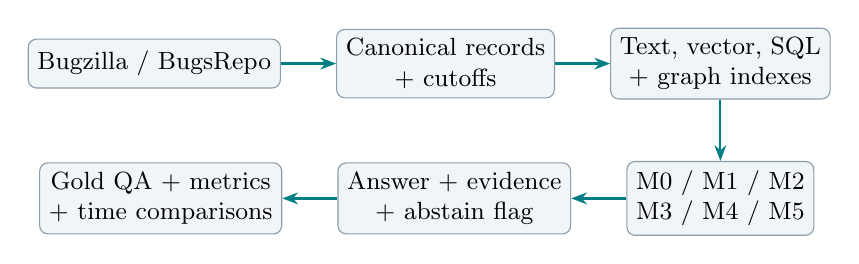
\begin{tikzpicture}[node distance=0.52cm and 0.7cm, every node/.style={font=\small},box/.style={draw=navy!50,rounded corners=3pt,fill=pale,minimum width=2.05cm,minimum height=0.62cm,align=center},arrow/.style={-{Stealth[length=2mm]},thick,draw=teal}]
\node[box] (raw) {Bugzilla / BugsRepo};
\node[box,right=of raw] (norm) {Canonical records\\+ cutoffs};
\node[box,right=of norm] (indexes) {Text, vector, SQL\\+ graph indexes};
\node[box,below=0.78cm of indexes] (methods) {M0 / M1 / M2\\M3 / M4 / M5};
\node[box,left=of methods] (answer) {Answer + evidence\\+ abstain flag};
\node[box,left=of answer] (eval) {Gold QA + metrics\\+ time comparisons};
\draw[arrow] (raw)--(norm); \draw[arrow](norm)--(indexes); \draw[arrow](indexes)--(methods); \draw[arrow](methods)--(answer); \draw[arrow](answer)--(eval);
\end{tikzpicture}
\end{center}

\subsection{Reproducibility and fairness controls}
\begin{itemize}
\item Same generation model and temperature for all generative arms; record API model ID and date (providers can silently change versions). Use distinct model names only as a \emph{secondary} robustness check.
\item Each arm gets the same maximum response length; M1/M2/M4 get identical maximum evidence-token budgets. M3 can consume only returned rows and its audit trace.
\item Log all retrieved chunk IDs and ranks, SQL-template names, selected bug records, prompt hashes, timestamps, retry history and latency. Cache responses by system/version/question to avoid unnecessary free-tier requests.
\item Separate retrieval comparison from response quality: report Recall@5/10 for retrievers and count evidence retrieval failures independently of generation failures.
\item No arbitrary shell, Python or SQL execution by the model. Only allowlisted, read-only parameterized SQL with resource/time limits. Treat bug text as untrusted instructions.
\end{itemize}

\section{Evaluation: correctness, hallucination and cost}
\subsection{What counts as correct?}
\begin{longtable}{@{}p{0.25\linewidth}p{0.65\linewidth}@{}}\toprule
\textbf{Family}&\textbf{Primary scoring rule}\\\midrule\endhead
Lookup (F1)&Exact normalized fields; timestamps normalized to UTC if used.\\
Lifecycle (F2)&Computed hours/days within predefined tolerance (e.g., $\pm 1$ hour only for rounded verbal answers); event type and reopen handling correct.\\
Aggregate (F3)&Exact integer count over the specified sampled corpus and cutoff; no unstated broader population.\\
Relationships (F4)&Set precision/recall/F1 for related IDs plus correct time-filtered status; count question correct only if complete.\\
Explanation (F5)&Human-graded: correct, partially supported or incorrect; every material causal claim mapped to a source comment.\\
Unanswerable (F6)&Correct abstention/qualified ``not available'' without inventing person-hours, source data or a closed state.\\\bottomrule
\end{longtable}

\textbf{Question-level primary accuracy:} binary \texttt{correct} after normalization for F1--F4 and F6; F5 correct iff all material claims are source-supported and address the requested issue. Also provide partial-credit breakdown, especially for F4 and F5.

\subsection{Hallucination and citation protocol}
Annotators segment responses into \emph{atomic checkable claims}: ``bug B was opened on date D'', ``its assigned engineer was P'', ``it was delayed due to test failures'', etc. Mark each as \texttt{supported}, \texttt{contradicted}, or \texttt{not verifiable from allowed evidence}; explicitly separate an \emph{answerability} error from a \emph{citation} error.
\begin{align*}
\text{Unsupported-claim rate} &= \frac{\#\text{contradicted or unsupported atomic claims}}{\#\text{all factual atomic claims}},\\
\text{Citation precision} &= \frac{\#\text{cited sources actually supporting claims}}{\#\text{all cited sources}},\\
\text{Correct abstention} &= \frac{\#\text{correct abstentions on unanswerable questions}}{\#\text{unanswerable questions}}.
\end{align*}
Also report the \emph{fraction of answers containing at least one unsupported claim}; a low claim rate may conceal a high affected-answer rate. A missing citation is an evidence defect but not automatically proof that an otherwise correct mathematical result is false.

\textbf{Judging:} automatically compute exact answers where possible; manually judge F5 and sample F1--F4; optionally use a \emph{separate} LLM judge on short claim/evidence pairs, blinded to method, then audit a stratified human subset. Report inter-rater agreement on 40 doubly reviewed responses; adjudicate conflicts. Never use the same unverified LLM judge's score as sole proof of no hallucinations.

\subsection{Statistical protocol}
Run all systems on identical test questions, compare paired correctness. Report Wilson 95\% intervals for individual success proportions and question-level bootstrap 95\% intervals for paired differences (resample question IDs, not retrieved chunks). With a small course-sized test, focus on effect sizes and uncertainty; avoid excessive per-cell significance claims. For F5, publish rubric and sample decisions. Record medians and p95 for wall-clock latency; separate local index build time from query time.

\section{Temporal updates and drift: the key experiment}
\subsection{Do not conflate two types of drift}
\textbf{Knowledge freshness} is when the required record was created or changed after a system's indexed snapshot. \textbf{Distribution shift} is when the style, components or mix of bug reports changes. A simple before/after data addition experiment primarily measures \emph{freshness/update handling}; do not call it model concept drift without further distributional evidence.

\subsection{Frozen snapshots and test conditions}
Set $T_0$ to a data-validated historical cutoff (ideally near BugsRepo's October 2024 coverage) and $T_1>T_0$ using verified later Bugzilla events. The exact dates are determined \emph{after the audit}; they should not be assumed from upload filenames alone.

\begin{tabularx}{\linewidth}{@{}p{0.24\linewidth}p{0.31\linewidth}X@{}}\toprule
\textbf{Condition}&\textbf{Accessible material}&\textbf{Purpose}\\\midrule
A: Historical&Only evidence available by $T_0$; questions as of $T_0$&Check ordinary correctness without future leakage.\\
B: Stale on new&Indexes/store frozen at $T_0$; questions requiring information through $T_1$&Measure missing-new-knowledge behavior; correct abstention may be optimal.\\
C: Refreshed&Ingest exactly the same new events/bugs through $T_1$ for all eligible methods&Measure update recovery under equal data access.\\
D: Fresh-only (optional)&Questions exclusively about $T_0<T\le T_1$ bugs and events&Stress-test truly newly introduced IDs and components.\\\bottomrule
\end{tabularx}

\textbf{Primary temporal metrics:} Accuracy\textsubscript{historical}, Accuracy\textsubscript{stale}, Accuracy\textsubscript{refreshed}; \emph{staleness penalty} $=A_{\mathrm{historical}}-A_{\mathrm{stale}}$ only on \emph{matched/equivalent} strata; \emph{refresh gain} $=A_{\mathrm{refreshed}}-A_{\mathrm{stale}}$ on identical $T_1$ questions. Do \emph{not} calculate a simple penalty between different easy/hard question sets and attribute it to drift. Show correct-abstention separately: stale systems should not be penalized for honestly saying that post-cutoff evidence is inaccessible in an evidence-bounded setting.

\textbf{Implementation:} new reports and changes are ingested once into \texttt{updates\_v1}; rebuilt or incremental BM25/FAISS indexes and SQL/graph tables are compared under a common manifest. Check for retroactively modified older bug records. Archive the exact update records so the experiment can be replayed offline.

\section{Zero-cost implementation choices}
\begin{longtable}{@{}p{0.25\linewidth}p{0.30\linewidth}p{0.36\linewidth}@{}}\toprule
\textbf{Need}&\textbf{Preferred free tool}&\textbf{Why / caveat}\\\midrule\endhead
Language model&Google AI Studio + Gemini API free-tier eligible \texttt{gemini-3.5-flash-lite} candidate\cite{geminipricing}&Current pricing shows free input/output for this model; \emph{check active model and RPM/TPM/RPD limits in your own account}. Free usage may be processed to improve Google products.\\
Offline LLM fallback&Ollama with a suitable quantized open-weight instruct model (e.g., Qwen family)&No API billing; depends on available VRAM/RAM, may yield different quality. Use \emph{the same chosen generator} for compared arms.\\
Local embeddings&\texttt{sentence-transformers}, \texttt{all-MiniLM-L6-v2}&No embedding API cost; simple, reproducible semantic baseline.\\
Keyword search&SQLite FTS5 or \texttt{rank-bm25}&Local exact/lexical matching.\\
Vector search&FAISS CPU (or local Chroma)&Local, adequate for thousands of chunks.\\
Structured analytical queries&DuckDB + Parquet; or SQLite&Free, direct aggregation and timestamp computation.\\
Graph&NetworkX on explicit bug relationships&Free, sufficient for small 1--2 hop neighborhoods.\\
Orchestration&Plain Python functions + Pydantic&Less moving machinery than agents/LangChain; transparent traces.\\
Interface&Streamlit&One-process localhost research demo.\\
Experiment tracking&CSV/JSONL, Git, \texttt{pytest}, scripts&Reproducibility without paid monitoring or deployment.\\
Charts&Matplotlib / seaborn-free plotting if preferred&Accuracy/CI by method/type, hallucinations, latency, update effects.\\\bottomrule
\end{longtable}

\textbf{Important billing distinction:} AI Studio's interactive playground is not a substitute for an \emph{API key} in a reproducible Python study. Use the official \texttt{google-genai} Python SDK\cite{geministart}; confirm the project is \texttt{Free} and \emph{do not enable billing}. A free model is subject to daily/request/token limits and availability may change; no particular call allowance is guaranteed. Send only public, minimized bug content, since Google's free tier may use submitted content to improve products\cite{geminipricing}.

\subsection{Budget discipline}
\begin{itemize}
\item Do all 180 ground-truth construction and retrieval tests \emph{without} the LLM whenever feasible. A four-arm, 144-test-question run involves roughly $4\times144=576$ answers before reruns (M0--M3); adding M4 makes 720. Free daily quotas may require controlled multi-day execution.
\item Cache embeddings and prompt responses to disk; run one low-volume dry run before full evaluation. Set output length limits, structured JSON responses, conservative retries on 429 and persistent progress checkpoints.
\item Keep \emph{one primary generator} fixed for all arms; a second model robustness test is optional and should not double the mandatory budget.
\item Avoid paid vector DBs, Neo4j Aura hosted billing, commercial LLM evaluators, crawler proxy services and full LLM-extracted graph construction.
\end{itemize}

\section{Concrete repository structure, commands and contracts}
\begin{lstlisting}
firefox-history-qa/
  README.md  pyproject.toml  .env.example  Makefile
  configs/{study.yaml,models.yaml}
  data/{raw/,normalized/,snapshots/,manifest.yaml}
  src/
    extract/{bugsrepo_import.py,bugzilla_client.py}
    normalize/{schema.py,events.py,snapshots.py}
    index/{bm25.py,dense.py,graph.py}
    methods/{blind.py,lexical_rag.py,hybrid_rag.py,
             sql_query.py,graph_retrieval.py,router.py}
    eval/{build_gold.py,run.py,score.py,judge.py,plots.py}
    app/streamlit_app.py
  benchmark/{dev.jsonl,test.jsonl,rubric.md}
  tests/{test_time_math.py,test_snapshots.py,test_sql.py}
  results/{runs/,tables/,plots/}
  reports/{literature_matrix.md,data_audit.md,final_report.tex}
\end{lstlisting}

\textbf{Setup commands (illustrative CLI contract---create these scripts first; not a claim they already exist):}
\begin{lstlisting}
python -m venv .venv
source .venv/bin/activate
pip install requests pandas pyarrow duckdb rank-bm25 faiss-cpu \
  sentence-transformers google-genai streamlit networkx \
  pydantic python-dotenv pytest matplotlib
cp .env.example .env   # Add GEMINI_API_KEY locally; never commit it
python -m src.extract.bugsrepo_import --manifest data/manifest.yaml
python -m src.extract.bugzilla_client --mode smoke --limit 50
python -m src.normalize.snapshots --cutoff <AUDITED_T0>
python -m src.eval.build_gold --split dev
python -m src.index.bm25 --snapshot v0
python -m src.index.dense --snapshot v0
python -m src.eval.run --split dev --method all --snapshot v0
pytest -q
streamlit run src/app/streamlit_app.py
\end{lstlisting}

\textbf{Unified model output schema:} \texttt{\{answer: string, abstained: bool, evidence: [\{bug\_id, record\_id, url\}], method: string, snapshot: string\}}. Store raw model text separately for auditing malformed JSON. Never let a parser failure masquerade as a correct abstention.

\subsection{Read-only SQL example and safety}
The \emph{real} SQL template depends on normalized events, but conceptually:
\begin{lstlisting}
SELECT b.bug_id,
       date_diff('hour', b.created_at,
         min(e.event_time)) AS hours_to_first_fixed
FROM bugs b JOIN fix_events e ON e.bug_id = b.bug_id
WHERE b.bug_id = ? AND e.event_time <= ?
GROUP BY b.bug_id, b.created_at;
\end{lstlisting}
\texttt{fix\_events} is a \emph{validated derived table} created only from qualifying FIXED state transitions; it is not all \texttt{RESOLVED} events. Parameterize IDs/times, enforce \texttt{SELECT}-only template IDs, timeouts and row limits. Test reopened/missing-history cases explicitly.

\section{Eight-week plan with dependencies and gates}
\begin{longtable}{@{}p{0.09\linewidth}p{0.42\linewidth}p{0.40\linewidth}@{}}\toprule
\textbf{Week}&\textbf{Tasks (in execution order)}&\textbf{Exit criterion / milestone}\\\midrule\endhead
\textbf{1}&Read RepoChat, Abedu TOSEM, BugsRepo, ticket KG+RAG. Agree RQs/metrics; inspect Zenodo files; clone and review mining scripts; test 50 API cases; choose single Bugzilla product scope.&One-page novelty matrix, written study protocol, working API smoke script; go/no-go on history availability.\\
\textbf{2}&Build import and REST downloader; normalize bugs/comments/events; audit coverage, duplicates and status variants; freeze $T_0$ and $T_1$; construct initial SQL tables.&Versioned data manifest and audited Parquet; 20 checked bugs with history; no future data in $T_0$.\\
\textbf{3}&Define scoring rubric and six families; generate candidate questions; review explanation answers; lock 36-dev/144-test split; test deterministic gold-answer calculations.&180 QA records with documented gold/support and question/bug split; benchmark freeze.\\
\textbf{4}&Implement M0 closed-book, M1 BM25, M2 hybrid with local embeddings, one common LLM wrapper; smoke test on development set.&Each system gives parseable response, source references and logs; retrieval Recall@k verified.\\
\textbf{5}&Implement M3 template-driven DuckDB, optional M4 NetworkX if on schedule; validate exact questions and no SQL leaks.&Lifecycle and aggregate unit tests pass; manual 10-bug check; parity of scope/time filters.\\
\textbf{6}&Run locked test once for all core methods under $T_0$; manually audit F5 and claim grounding; gather output JSONL; render first tables.&Per-family outcome table, unsupported-claim and abstention results, paired intervals.\\
\textbf{7}&Run A/B/C update protocol; measure refresh gain; inspect 10--15 failure cases; if ahead, run M4 or M5 router experiment.&Temporal ablation results with immutable manifests and evidence of actual new events.\\
\textbf{8}&Build Streamlit demonstration; write report and limitations; independent rerun from clean instructions; rehearse presentation.&All D1--D8 present; report tables reproducible from raw run files; working live demo + recorded fallback.\\\bottomrule
\end{longtable}

\textbf{Six-week compression:} combine weeks 1--2 and 7--8, \emph{drop M4/M5}, reduce corpus size, but keep locked benchmark, deterministic QA, temporal protocol and hallucination scoring. The primary four-arm study survives; the graph becomes future work rather than an unsupported claim.

\subsection{How to divide responsibilities (team of three or four)}
\begin{itemize}
\item \textbf{Data lead:} mining, normalization, time reconstruction, SQL gold computations, manifest.
\item \textbf{Systems lead:} LLM interface, BM25/vector indexes, M0--M3 implementation, optional graph.
\item \textbf{Evaluation lead:} question taxonomy, annotation, pairwise experiments, statistics, leakage audits.
\item \textbf{Optional fourth member:} demo UI, integration tests, report assembly; also independently review annotations.
\end{itemize}
\textbf{Team synchronization:} merge first against frozen interfaces and example JSON; two short meetings weekly; no simultaneous edits to the locked test benchmark. Everyone reviews some gold examples before comparing systems.

\section{Risk register and fallback decisions}
\begin{longtable}{@{}p{0.29\linewidth}p{0.44\linewidth}p{0.17\linewidth}@{}}\toprule
\textbf{Risk}&\textbf{Mitigation / fallback}&\textbf{Priority}\\\midrule\endhead
BugsRepo comments too large, duplicated or schema inconsistent&Read only required CSV slices, hash/ID dedup, audit sampling, retrieve extra histories for benchmark IDs.&High\\
Missing status-transition histories&Limit F2/reopen items to validated API history; do not infer fix time from last-change time.&Critical\\
Free API quota reached or rate limited&Resume jobs with checkpoints, use local quantized LLM if practical, narrow run, do not pay or bypass provider limits.&High\\
LLM returns invalid graph/SQL tool calls&Use typed JSON intents and allowlisted SQL templates; record parse errors separately.&High\\
Temporal leakage through current API fields&Materialize snapshots by event time plus evidence availability; explicit cutoff unit tests and manual audits.&Critical\\
LLM evaluation unreliable&Use deterministic answers + source-level human annotation; calibrate any LLM-assisted judge.&High\\
One approach is clearly worse&Report honestly, analyze question subtypes and failure mechanisms; no benchmark cherry-picking.&Normal\\
No time for graph construction&Run M0--M3 only; cite existing KG work as background; optional graph remains a stretch objective.&Normal\\
Public records include email/user data&Minimize stored identity fields; pseudonymize contributor IDs, avoid pasting personal data into public model inputs; follow source reuse terms.&High\\
\bottomrule\end{longtable}

\section{What results will be persuasive?}
The project should end with a \textbf{method $\times$ question-family} correctness matrix, a per-method hallucination/abstention table, a retrieval-quality plot, a latency plot, and a paired freshness/refresh comparison. Show the number of test items per cell and confidence intervals. \emph{Do not invent expected accuracy numbers} before running the models.

\textbf{Illustrative interpretation patterns (not predictions):}
\begin{itemize}
\item If SQL excels at F2/F3 but cannot answer F5, the key insight is the need to separate calculation from language synthesis.
\item If M2 retrieves the right comment but fabricates a developer motive, retrieval is not sufficient for grounded generation.
\item If M4 helps F4 but not F1, relationships have selective value rather than universal benefit.
\item If a stale system abstains and refreshed systems answer correctly, differentiate \emph{safe ignorance} from \emph{hallucinated confidence}.
\item If a generic model happens to answer old famous Firefox bugs correctly, exclude shared public bug IDs in a sensitivity analysis rather than calling closed-book recall universally reliable.
\end{itemize}

\section{First 72 hours: a precise action checklist}
\begin{enumerate}
\item \textbf{Create a Git repository} with project structure, \texttt{README}, issue board, and a one-page scope/terms document; choose $T_0$ only after inspecting actual dataset dates.
\item \textbf{Read and annotate} RepoChat (2025), Abedu TOSEM (2026), BugsRepo (2025); explicitly describe the novelty boundary.
\item \textbf{Download a small sample,} e.g., BugsRepo's sample/structured CSV, not every 4.3-GB file. Inspect at least 20 rows and the documented identical comments-file MD5s.
\item \textbf{Test REST endpoints} for 50 sampled bugs; verify \texttt{creation\_time}, comments and the \texttt{history} field; inspect reopen and non-FIXED cases.
\item \textbf{Write five gold questions manually} covering lookup, duration, aggregate, relation and unanswerable; validate answers against the source.
\item \textbf{Produce a minimum vertical slice:} type a bug ID/question $\rightarrow$ fetch normalized records $\rightarrow$ deterministic computed fact $\rightarrow$ displayed answer plus provenance. This is the best early demo.
\end{enumerate}

\begin{keybox}
\textbf{Decision after 72 hours:} If histories are consistently accessible and a 50-bug sample can be normalized, proceed with the plan. If not, restrict the benchmark to fields with verified provenance and treat lifecycle/duration questions as a limited subset; \emph{do not fabricate historical events to make the original proposal work}.
\end{keybox}

\section{Suggested final report outline and demo}
\textbf{Report:} (1) Problem and contribution; (2) related work and non-novelty boundaries; (3) data collection and ethical considerations; (4) schema/time semantics; (5) question benchmark and annotation; (6) systems and matched controls; (7) evaluation metrics and paired statistics; (8) results by question family; (9) temporal updates; (10) hallucination examples and limitations; (11) threats to validity; (12) conclusion and reproduction checklist.

\textbf{Five-minute demo:} Ask one factual duration question where SQL returns an exact event-derived number, one explanation question with comment citations, one impossible engineer-hours question that should abstain, and one new-bug question demonstrating a frozen versus refreshed index. Show the source record and selected snapshot clearly. Use a recorded demo fallback in case a free-tier key is throttled during the presentation.

\section{Research links and primary documentation}
All links below were checked during preparation; they are starting points, not a guarantee that external services or free quotas will remain unchanged.
\begin{thebibliography}{99}\setlength{\itemsep}{3pt}
\bibitem{bugsrepo} J. Acharya and G. Ginde, ``BugsRepo: A Comprehensive Curated Dataset of Bug Reports, Comments and Contributors Information from Bugzilla,'' \emph{Proc. EASE}, 2025. \url{https://arxiv.org/abs/2504.18806}. Published dataset: \url{https://zenodo.org/records/15004067}; code: \url{https://github.com/GindeLab/EASE_2025_Data_paper}.
\bibitem{zenodo} Acharya and Ginde, ``EASE 2025 Dataset (BugRepo),'' Zenodo record 15004067 (file list, sizes and MD5 checksums). \url{https://doi.org/10.5281/zenodo.15004067}.
\bibitem{bugzillaapi} Bugzilla, ``Bug REST API: Get Bug; History; Search Bugs,'' official documentation. \url{https://bugzilla.readthedocs.io/en/latest/api/core/v1/bug.html}. See also comments endpoint: \url{https://bugzilla.readthedocs.io/en/latest/api/core/v1/comment.html}.
\bibitem{repochat} S. Abedu et al., ``RepoChat: An LLM-Powered Chatbot for GitHub Repository Question-Answering,'' \emph{MSR}, 2025. \url{https://2025.msrconf.org/details/msr-2025-data-and-tool-showcase-track/35/RepoChat-An-LLM-Powered-Chatbot-for-GitHub-Repository-Question-Answering}; code: \url{https://github.com/sabedu/repositoryChat}.
\bibitem{abedu} S. Abedu, S. Khatoonabadi, and E. Shihab, ``Synergizing LLMs and Knowledge Graphs: A Novel Approach to Software Repository-Related Question Answering,'' \emph{ACM TOSEM}, 2026. \url{https://arxiv.org/abs/2412.03815}; code: \url{https://github.com/sabedu/knowledge_graph_llm_synergy}.
\bibitem{xukgrag} Z. Xu et al., ``Retrieval-Augmented Generation with Knowledge Graphs for Customer Service Question Answering,'' 2024. \url{https://arxiv.org/abs/2404.17723}.
\bibitem{edgerag} D. Edge et al., ``From Local to Global: A Graph RAG Approach to Query-Focused Summarization,'' 2024. \url{https://arxiv.org/abs/2404.16130}.
\bibitem{temporalkg} M. Su et al., ``Temporal Knowledge Graph Question Answering: A Survey,'' 2024. \url{https://arxiv.org/abs/2406.14191}.
\bibitem{ragas} S. Es et al., ``RAGAS: Automated Evaluation of Retrieval Augmented Generation,'' 2023. \url{https://arxiv.org/abs/2309.15217}.
\bibitem{geminipricing} Google AI for Developers, ``Gemini Developer API pricing,'' retrieved October 2026. \url{https://ai.google.dev/gemini-api/docs/pricing}. Quotas: \url{https://ai.google.dev/gemini-api/docs/rate-limits}.
\bibitem{geministart} Google AI for Developers, ``Getting started with Gemini API (Python),'' \url{https://ai.google.dev/gemini-api/docs/get-started}.
\bibitem{minilm} Sentence Transformers, ``all-MiniLM-L6-v2 model card,'' \url{https://huggingface.co/sentence-transformers/all-MiniLM-L6-v2}.
\end{thebibliography}
\vfill
\begin{center}\small\color{muted}Prepared as an executable course-project plan. Experimental results remain to be collected and validated.\end{center}
\end{document}